\documentclass[10pt,a4paper]{article}
\usepackage[utf8]{inputenc}

\usepackage{amsmath}
\usepackage{amsfonts}
\usepackage{amssymb}
\usepackage{graphicx}
\usepackage{listings}

\lstset{numbers=left,
	title=\lstname,
	numberstyle=\tiny, 
	breaklines=true,
	tabsize=4,
	language=Python,
	morekeywords={with,super,as},,
	frame=single,
	basicstyle=\footnotesize\tt,
	commentstyle=\color{comment},
	keywordstyle=\color{keyword},
	stringstyle=\color{string},
	backgroundcolor=\color{background},
	showstringspaces=false,
	numbers=left,
	numbersep=5pt,
	literate=
		{�}{{\ae}}1
		{�}{{\aa}}1
		{�}{{\o}}1
		{�}{{\AE}}1
		{�}{{\AA}}1
		{�}{{\O}}1
	}
\usepackage{setspace}
\doublespacing
\usepackage{bm}
\usepackage{hyperref}

\begin{document}'
\begin{center}
{\LARGE\bf
FYS4150\\
Project 2, deadline October 2.
}
 
\includegraphics[scale=0.1]{uio.png}\\
Authors: Robin D. Kifle, Sander W. Losnedahl and Vemund S. Thorkildsen\\
University of Oslo, Autumn 2017
 
{\LARGE\bf Abstract}
\end{center}
\newpage

\begin{center}
{\LARGE\bf Introduction}
\end{center}
The problem we will deal with in this project is of quantum mechanical nature. As none of the three authors have had any quantum mechanics courses we will focus on the mathematical and numerical side of this problem. In this project we are going to develop our own eigenvalue-solver by using Jacobi's method. We will study two different cases, the first is for one electron moving in a harmonic oscillator. The second case is for two electrons moving in a harmonic oscillator with and without repulsive coulomb interaction.  
\newpage'

\begin{center}
{\LARGE\bf Method}
\end{center} 
To create our eigenvalue solver we first have to take a look at the matrix at hand, to get an understanding of the problem.

$$
  -\frac{d^2}{d\rho^2} u(\rho) + \rho^2u(\rho)  = \lambda u(\rho) .
$$

\noindent This equation will be solved numerically, and has given eigenvalues $\lambda_0=3$, $\lambda_1=7$ and $\lambda_2=11$. We can use the expression for the second derivative to rewrite this. This expression is in our case given by:

$$
 u''=\frac{u(\rho+h) -2u(\rho) +u(\rho-h)}{h^2} +O(h^2)
$$ 
\noindent
The last part of this expression, namely $O(h^2$, is the truncation error and will not be used further. By using the first part, our expression now looks like this:

$$
\frac{-u(\rho_i+h) +2u(\rho_i) -u(\rho_i-h)}{h^2}+\rho_i^2u(\rho_i)  = \lambda u(\rho_i)
$$ 

$$
\frac{-u_{i+1} +2u_i -u_{i-1}}{h^2}+\rho_i^2u_i= \lambda u_i
$$

\noindent Our $h$ is given by $h=\frac{\rho_n - \rho_0}{n}$, as we want our $\rho_i$ to vary with step length $h$. By using this $h$, $\rho_i$ will take the form: $\rho_i = \rho_o + ih$. The oscillator potential is given by $(\rho_i)^2$ and will be denoted as $V_i$ in the rest of this article. Now we have everything we need to rearrange this problem as a a matrix eigenvalue problem. \\
\\
From our expression it is easy to see that the matrix we are looking for takes the negative of element $i+1$ and $i-1$, divided by the step length squared. It also need to take two times the positive of element $i$ divided by $h^2$ plus element $i$ multiplied by the oscillator potential $V_i$. This means that we are once again faced by a problem that involves a tridiagonal matrix. 

\begin{center}
Main diagonal = $\frac{2}{h^2} + V_i$, first diagonal above and below = $-\frac{1}{h^2}$
\end{center}

\noindent On matrix form this looks like:

\begin{center}


$
 \begin{bmatrix} 
 \frac{2}{h^2}+V_1 & -\frac{1}{h^2} & 0   & 0    & \dots  &0     & 0 \\
 -\frac{1}{h^2} & \frac{2}{h^2}+V_2 & -\frac{1}{h^2} & 0    & \dots  &0     &0 \\
  0   & -\frac{1}{h^2} & \frac{2}{h^2}+V_3 & -\frac{1}{h^2}  &0       &\dots & 0\\
  \dots  & \dots & \dots & \dots  &\dots      &\dots & \dots\\
  0   & \dots & \dots & \dots  &\dots  &\dots & \dots\\
 0   & \dots & \dots & \dots  &\dots       & \dots & \frac{2}{h^2}+V_{N-1}
             \end{bmatrix} 
             \begin{bmatrix}
             u_0\\
             u_1\\
             u_2\\
             \dots\\
             \dots\\
             u_n\\
             \end{bmatrix} =\lambda
             \begin{bmatrix}
              u_0\\
             u_1\\
             u_2\\
             \dots\\
             \dots\\
             u_n\\
             \end{bmatrix}
$
\end{center}
We are going to solve this by using a Jacobi rotation algorithm. This uses a lot of similarity transformations. As long as:
$$v_j^Tv_i=\delta_{i j}$$
$$U^TU=I$$
The transformations can be shown to preserve the dot product and orthogonality by multiplying with the transpose of the matrix:
$$w=Uv$$
$$w^Tw=(Uv)^TUv=v^TU^TUv=v^Tv=\delta_{i j}$$

\noindent As stated earlier in this article we are going to solve this problem by using the Jacobi eigenvalue algorithm. Consider a symmetric matrix A and Givens rotation matrix R:
$$A'=RAR^T$$
$A'$ is symmetric and similar. $A'$ has entries:
$$A'_{ii} = c^2A_{ii}-2scA_{ij}+s^2A{jj}$$
$$A'_{jj} = s^2A_{ii}+2scA_{ij}+c^2A_{jj}$$
$$A'_{ij} = A'_{ji} = (c^2-s^2)A_{ij}+sc(A_{ii}-A_{jj})$$
$$A'_{ik}=A'_{ki}=cA_ik-sA_{jk} \hspace{3cm} k\neq i,j$$
$$A'_{jk} = A'_{kj} = sA_{ik}+cA_{jk} \hspace{3cm} k\neq i,j$$
$$A'_{kl} = S_{kl} \hspace{5cm} k,l \neq i,j$$
where $s=sin(\theta)$ and $c=cos(\theta)$
We choose $\theta$ such that $A'_{ij}=0$
Rewrite the 3rd equation:
$$A'_{ij}=c(2\theta)A_{ij}+\frac{1}{2}s(2\theta)(A_{ii}-A_{jj})$$
And set this equal to zero:
$$t(2\theta)=\frac{2A_{ij}}{A_{jj}-A_{ii}}$$
if $A_{jj}=A_{ii}$, then $\theta=\frac{\pi}{4}$
This is optimized by using the off-diagonal element with the largest absolute value as $A_{ij}$
The Jacobi eigenvalue method repeats this rotation until the matrix becomes close to diagonal. The elements on the diagonal are then approximations of the real eigenvalues of $A$.

\newpage

\begin{center}
{\LARGE\bf Results}
\end{center}
We have run our algorithm for different cases and focused on different parameters. The different cases have been for two electrons with and without repulsive coulomb interaction. In the first four figures we have focused on the eigenvalues created by the eigenvalue solver. This has been plotted against the number of iterations $n$ for 4 different values of ${\rho}_{max}$. This is compared to the known values of the three lowest eigenvalues, $\lambda_1=3$, $\lambda_2=7$, $\lambda_3=11$, to find a sensible value of ${\rho}_{max}$. 

\begin{center}
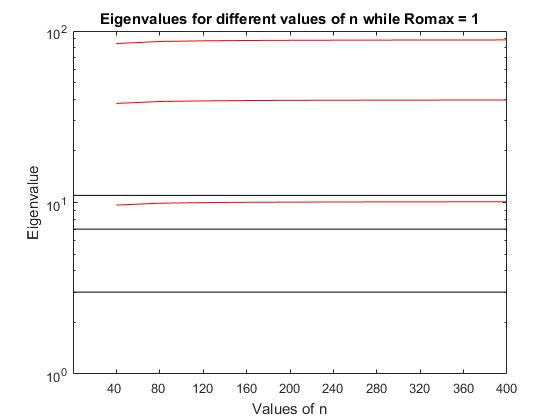
\includegraphics[scale=0.65]{rho1.jpg}

$Figure-1$: Here we have chosen ${\rho}_{max}$ to be 1. As the three lowest eigenvalues are known, this is obviously not a good fit.   



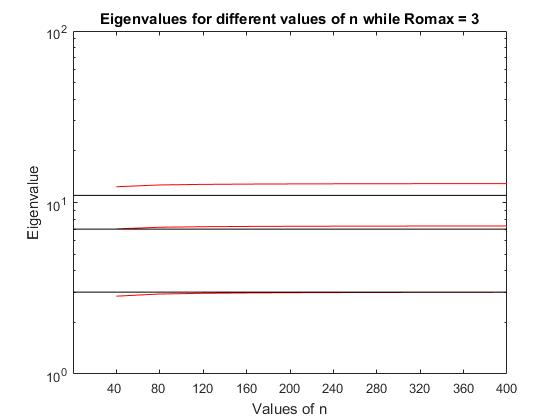
\includegraphics[scale=0.55]{rho3.jpg}

$Figure-2$: Here we have chosen ${\rho}_{max}$ to be 3. The eigenvalues are much closer than in figure 1, but they are still not correct. 


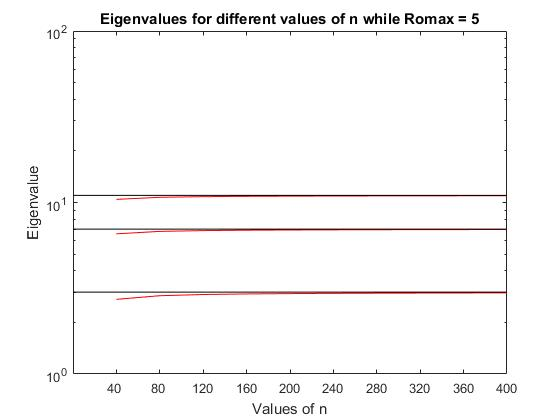
\includegraphics[scale=0.55]{rho5.jpg}
$Figure-3$: Here we have chosen ${\rho}_{max}$ to be 5. In this case all the eigenvalues converge to the correct values. 

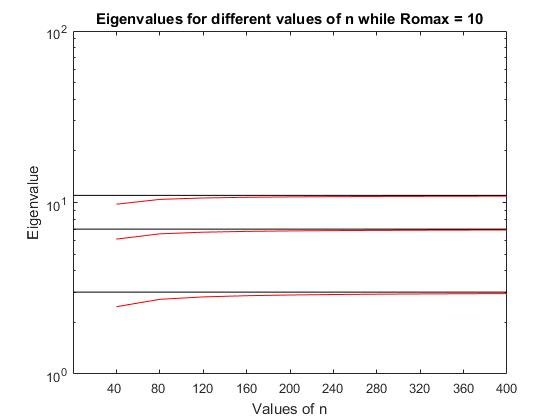
\includegraphics[scale=0.6]{rho10.jpg}
$Figure-4$: Here we have chosen ${\rho}_{max}$ to be 10. In this case all the eigenvalues converge to the correct values, but slower than in the case with ${\rho}_{max}=5$
\end{center}

\noindent From these plots it is easy to see that ${\rho}_{max}=1$ and ${\rho}_{max}=3$ is to low( Figure 1, Figure 2), while the two larger values seem to produce the correct results (Figure 3, Figure 4). The reason for this will be discussed later in the article. Now we can plot the wave functions produced by the same runs, i.e the case with 2 non-interacting electrons. 
\newpage
\begin{center}
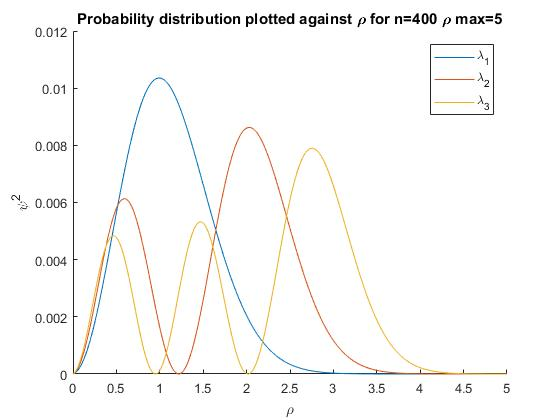
\includegraphics[scale=0.55]{eig400rho5.jpg}
$Figure-5$: Here we have chosen ${\rho}_{max}$ to be 5. The probability dies out before we reach ${\rho}_{max}$. We also see that $\lambda_1$ only has one top, $\lambda_2$ has two tops and $\lambda_3$ has three tops. 

\includegraphics[scale=0.55]{eig360Rho10.jpg}
$Figure-6$: Here we have chosen ${\rho}_{max}$ to be 10. The wave function is of similar shape, and dies out at the approximately the same place as for ${\rho}_{max}=5$. 
\end{center}

\noindent As the wave function dies out at approximately the same place in both Figure 5 and Figure 6, the most sensible ${\rho}_{max}$ will be 5. 









\newpage

\begin{center}
{\LARGE\bf Discussion}
\end{center}
\newpage

\begin{center}
{\LARGE\bf Concluding remarks}
\end{center}
\end{document}